% 2008 年广东卷理科第 20 题：四棱锥 P-ABCD，底面 ABCD 是半径为 R 的圆的内接四边形，
%   BD 是圆的直径，∠ABD=60°，∠BDC=45°，PD⊥底面 ABCD，PD=2√2R；
%   E、F 分别在 PB、CD 上且 PE/EB=DF/FC，过 E 作 BC 的平行线交 PC 于 G。
% 来源 PDF：gaokaomath-src/普通高考/2008/2008广东理.pdf
% SHA-256：c395b9608135bcd958aa64c448dfc14a8ba00fbc84cd20c3f1ad316e94d549b3
% 原页：2008广东理.pdf 第 2 页（A3 三栏）第 2 栏，书页码 446。
% 重绘依据：底面圆画成椭圆（前半实线、后半虚线），A 左、B 左下、C 下、D 右；
%   PD 竖直，P 位于 D 正上方；E 在 PB 上、G 在 PC 上且 EG∥BC，F 在 CD 上；
%   AD、BD、EF 被遮挡用虚线。
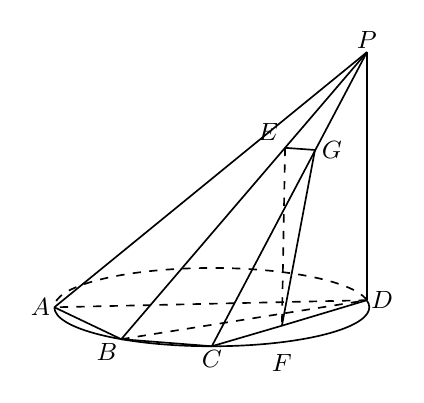
\begin{tikzpicture}[x=1.0cm, y=0.90cm, semithick, font=\small,
  every node/.style={inner sep=1.2pt}]
  % 底面椭圆：中心 (2.60,1.00)，半长轴 2.00、半短轴 0.55
  \coordinate (A) at (0.60,1.00);
  \coordinate (B) at (1.45,0.55);
  \coordinate (C) at (2.60,0.45);
  \coordinate (D) at (4.57,1.10);
  \coordinate (P) at (4.57,4.60);
  \coordinate (E) at (3.53,3.25);
  \coordinate (G) at (3.91,3.22);
  \coordinate (F) at (3.49,0.74);

  % 底面椭圆：后半（D→上→A）虚线，前半（A→下→D）实线
  \draw[dashed] (D) arc[start angle=10, end angle=180, x radius=2.00, y radius=0.55];
  \draw (A) arc[start angle=180, end angle=370, x radius=2.00, y radius=0.55];

  % 底面的边与对角线
  \draw (A) -- (B) -- (C) -- (F) -- (D);
  \draw[dashed] (D) -- (A);
  \draw[dashed] (B) -- (D);

  % 侧棱
  \draw (P) -- (A);
  \draw (P) -- (B);
  \draw (P) -- (C);
  \draw (P) -- (D);

  % 截面三角形 EFG
  \draw (E) -- (G);
  \draw (G) -- (F);
  \draw[dashed] (E) -- (F);

  \node[above] at (P) {$P$};
  \node[left] at (A) {$A$};
  \node[below left] at (B) {$B$};
  \node[below] at (C) {$C$};
  \node[right] at (D) {$D$};
  \node[above left=1pt] at (E) {$E$};
  \node[right=1pt] at (G) {$G$};
  \node[below=9pt] at (F) {$F$};
\end{tikzpicture}
